\section{Codifica}
\subsection{Interfaccie}
\subsubsection{Menù}
Viene mostrata il menù del ristorante che comprende tutte le categorie e le loro piatti.\\
\textbf{Funzionalità:}
\begin{itemize}
    \item L'utente può aumentare la quantità di un piatto per aggiungerlo o aumentare la sua quantità nell'ordine del tavolo;
    \item L'utente può diminuire la quantità di un piatto per rimuoverlo o diminuire la sua quantità nell'ordine del tavolo;
    \item L'utente può visualizzare il piatto in modalità dettaglio per dare una recensione al piatto o inserisce una nota per il piatto;
    \item L'utente può aggiungere il piatto nella lista dei preferiti o rimuoverlo dalla lista.
\end{itemize}
\begin{figure}[H]
    \centering
    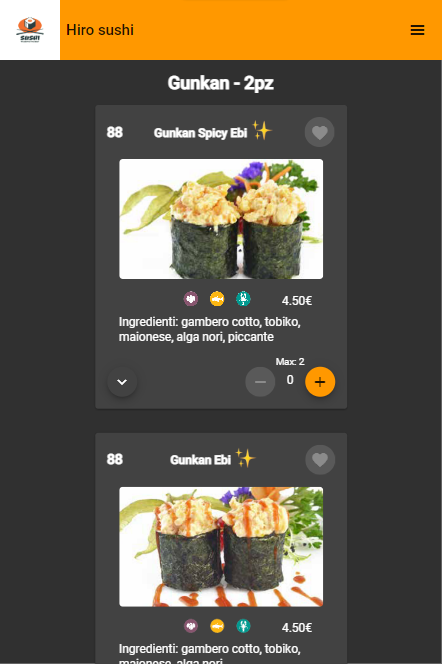
\includegraphics[scale=.6]{menu.png}
    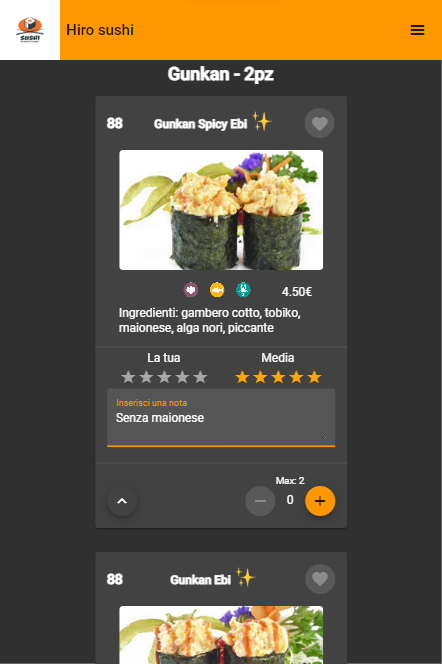
\includegraphics[scale=.6]{menu2.png}
    \caption{Menù e Menù con piatto in dettaglio di SushiLab}
\end{figure}
\pagebreak

\subsubsection{Gestione tavolo}
Viene mostrata la maschera di gestione tavolo.\\
\textbf{Funzionalità:}
\begin{itemize}
    \item L'utente può creare una sessione di tavolo;
    \item L'utente può andare al form per unire ad una sessione.
\end{itemize}
\begin{figure}[H]
    \centering
    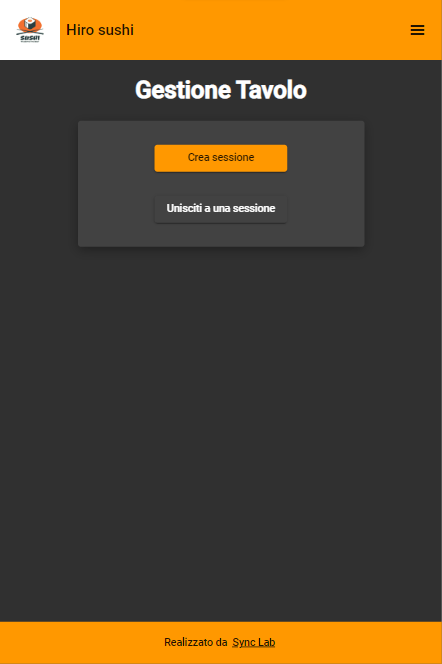
\includegraphics[scale=.6]{gestione tavolo.png}
    \caption{Maschera gestione tavolo SushiLab}
\end{figure}
\pagebreak

\subsubsection{Unisci sessione}
Interfaccia tramite la quale è possibile unire ad una sessione di tavolo.\\
\textbf{Funzionalità:}
\begin{itemize}
    \item L'utente può  unirsi ad una sessione inserendo il codice di sessione se il codice non rispetta la validazione del form non si abilita il bottone unisci;
    \item L'utente può tornare nella pagina gestione tavolo.
\end{itemize}
\begin{figure}[H]
    \centering
    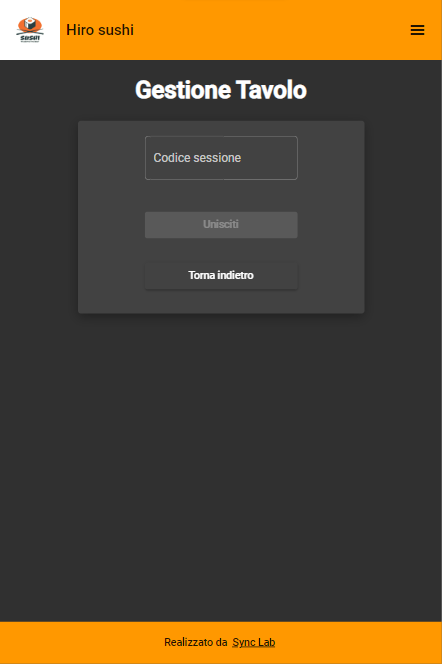
\includegraphics[scale=.6]{unisci.png}
    \caption{Maschera unisci sessione SushiLab}
\end{figure}
\pagebreak

\subsubsection{QR-code tavolo}
Viene mostrata il QR-code del tavolo che permette agli altri utenti che si trovano sullo stesso tavolo dell'untente di unirsi.\\
\textbf{Funzionalità:}
\begin{itemize}
    \item L'utente può uscire dalla sessione premendo il bottone esci dalla sessione.
\end{itemize}
\begin{figure}[H]
    \centering
    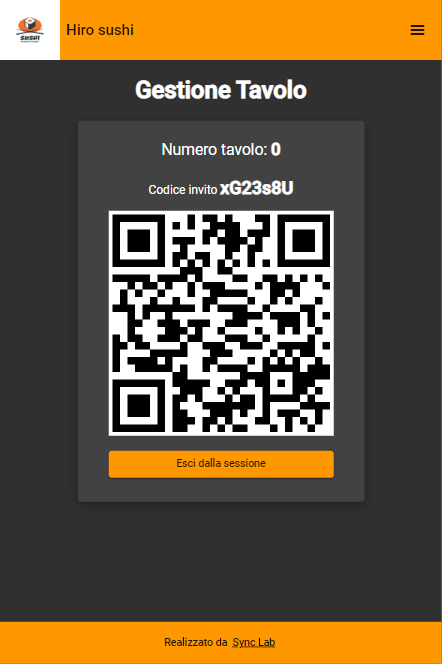
\includegraphics[scale=.6]{gestionetavolo2.png}
    \caption{Maschera QR-code tavolo SushiLab}
\end{figure}
\pagebreak

\subsubsection{Lista ordini del tavolo}
Viene mostrato la lista degli ordini della sessione del tavolo in cui si trova l'utente.\\
\textbf{Funzionalità:}
\begin{itemize}
    \item L'utente può spostare la lista in arrivo;
    \item L'utente può generare il QR-code premendo sul bottone QR-code;
    \item L'utente può andare in altri sezioni della lista ordini utilizzando la navbar interna.
\end{itemize}
\begin{figure}[H]
    \centering
    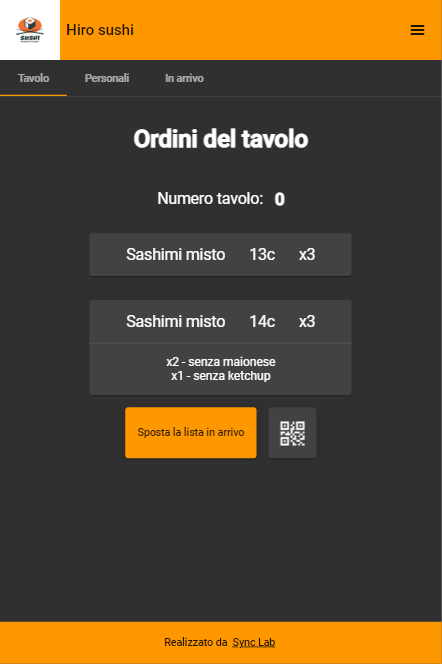
\includegraphics[scale=.6]{ordinitavolo.png}
    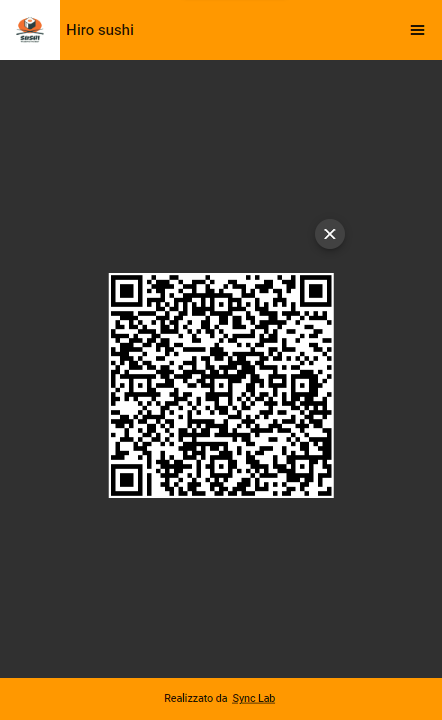
\includegraphics[scale=.6]{ordinitavolo2.png}
    \caption{Maschera lista ordini del tavolo e QR-code ordini SushiLab}
\end{figure}
\pagebreak

\subsubsection{Lista ordini personali}
Viene mostrata la lista degli ordini personali.\\
\textbf{Funzionalità:}
\begin{itemize}
    \item L'utente può visualizzare i piatti in modalità dettaglio;
    \item L'utente può visualizzare i piatti in modalità normale;
    \item L'utente può aggiungere un piatto nella lista dei preferiti o rimuoverlo dalla lista;
    \item L'utente può dare una recensione ad un piatto.
\end{itemize}
\begin{figure}[H]
    \centering
    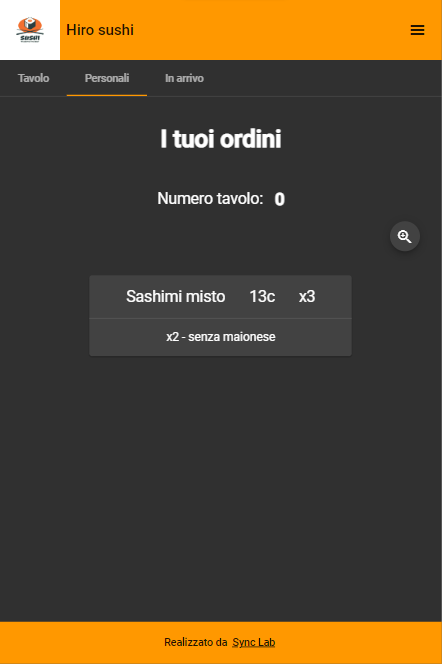
\includegraphics[scale=.6]{ordinipersonali.png}
    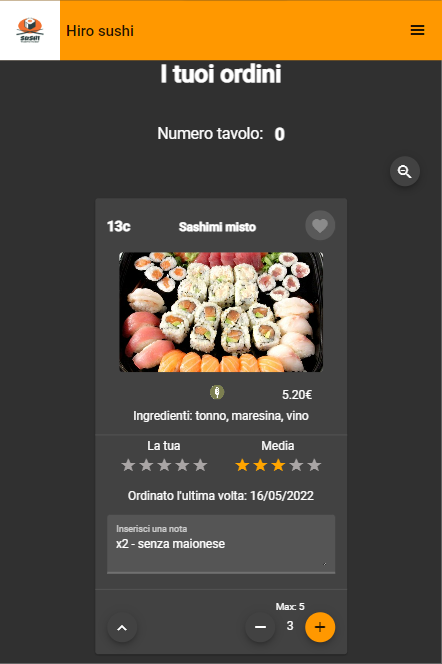
\includegraphics[scale=.6]{ordinipersonali2.png}
    \caption{Maschera ordini personali e ordini personali con piatti in dettaglio SushiLab}
\end{figure}
\pagebreak

\subsubsection{Lista ordini in arrivo}
Viene mostrata la lista degli ordini in arrivo.\\
\textbf{Funzionalità:}
\begin{itemize}
    \item L'utente può visualizzare i piatti in modalità dettaglio;
    \item L'utente può visualizzare i piatti in modalità normale;
    \item L'utente può marcare un piatto come arrivato;
    \item L'utente può aggiungere un piatto nella lista dei preferiti o rimuoverlo dalla lista;
    \item L'utente può dare una recensione ad un piatto.
\end{itemize}
\begin{figure}[H]
    \centering
    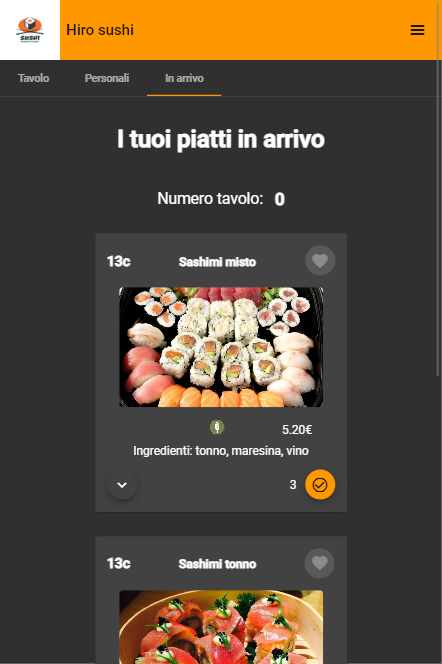
\includegraphics[scale=.6]{ordiniinarrivo.png}
    \caption{Maschera ordini in arrivo SushiLab}
\end{figure}
\pagebreak

\subsubsection{Login}
Viene mostrato il form per effetture il login dove è possibile effettuare la login nella piattaforma.\\
\textbf{Funzionalità:}
\begin{itemize}
    \item L'utente può effettuare il login inserendo i campi correttamente altrimenti viene evidenziato in rosso i campi sbagliati;
    \item L'utente può andare al form di registrazione;
    \item L'utente può andare al form di password dimenticata.
\end{itemize}
\begin{figure}[H]
    \centering
    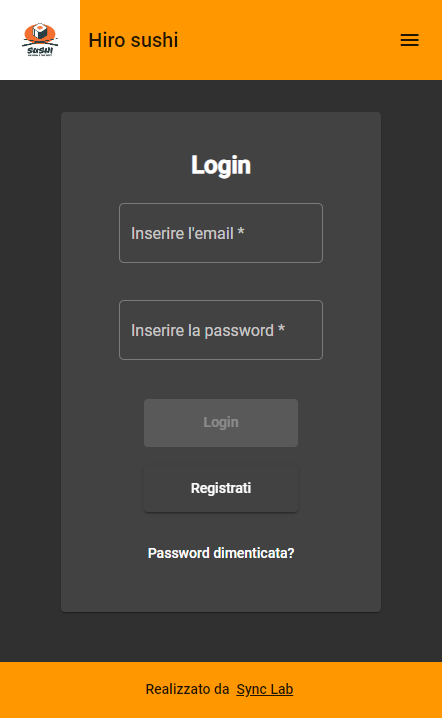
\includegraphics[scale=.6]{login.png}
    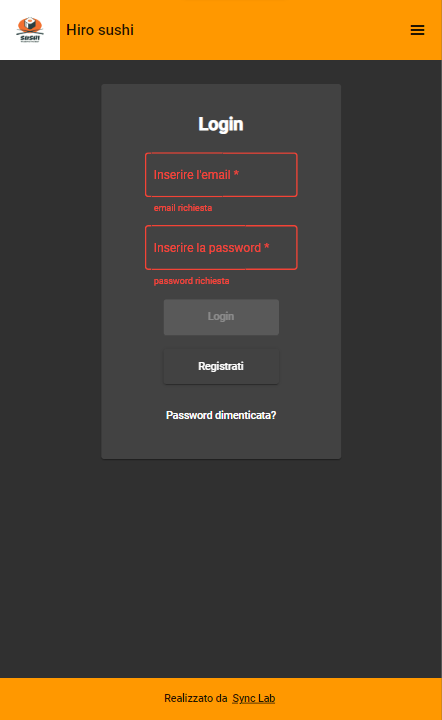
\includegraphics[scale=.6]{login2.png}
    \caption{Maschera login e login con campi errati SushiLab}
\end{figure}
\pagebreak

\subsubsection{Registrazione}
Viene mostrato il form di registrazione dove è possibile registrare nella piattaforma.\\
\textbf{Funzionalità:}
\begin{itemize}
    \item L'utente può effettuare la registrazione inserendo i campi correttamente altrimenti viene evidenziato in rosso i campi sbagliati;
    \item L'utente può andare al form di login.
\end{itemize}
\begin{figure}[H]
    \centering
    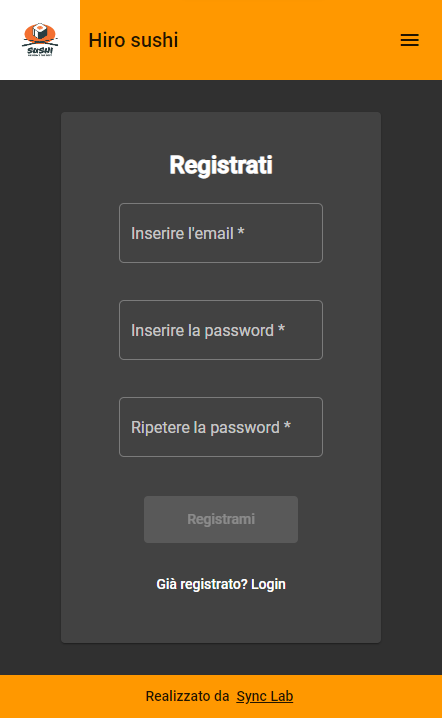
\includegraphics[scale=.6]{registrati.png}
    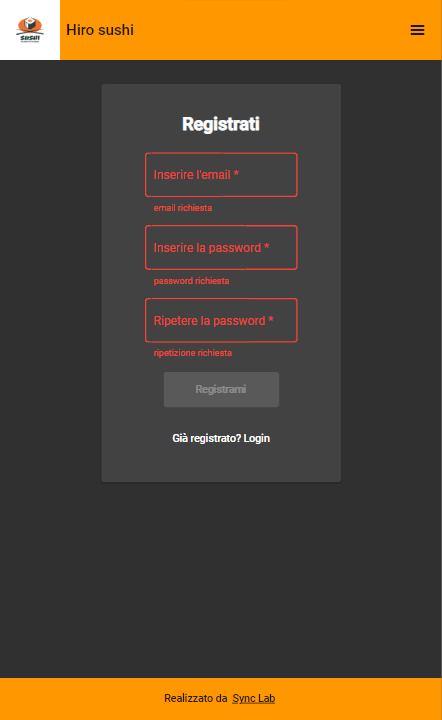
\includegraphics[scale=.6]{registrati2.png}
    \caption{Maschera registrazione e registrazione con campi errati SushiLab}
\end{figure}
\pagebreak

\subsubsection{Password Dimenticata}
Viene mostrato il form di cambia password dove è possibile reimpostare la password.\\
\textbf{Funzionalità:}
\begin{itemize}
    \setlength\itemsep{.1em}
    \item L'utente può reimpostare la password inserendo i campi correttamente altrimenti viene evidenziato in rosso i campi sbagliati;
    \item L'utente può andare al form di registrazione;
    \item L'utente può andare al form di Login.
\end{itemize}
\begin{figure}[H]
    \centering
    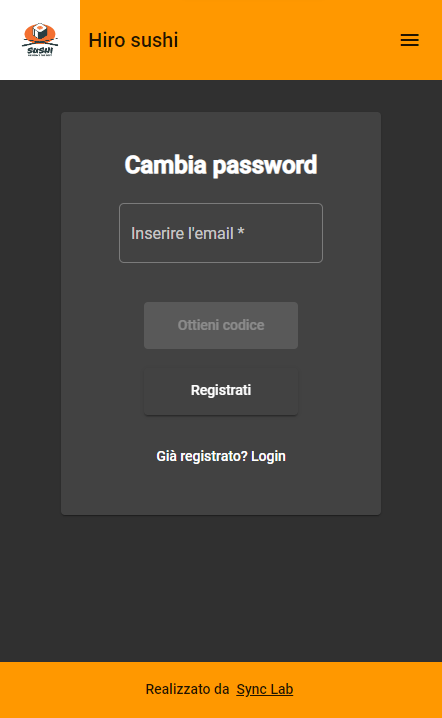
\includegraphics[scale=.5]{cambiapass.png}
    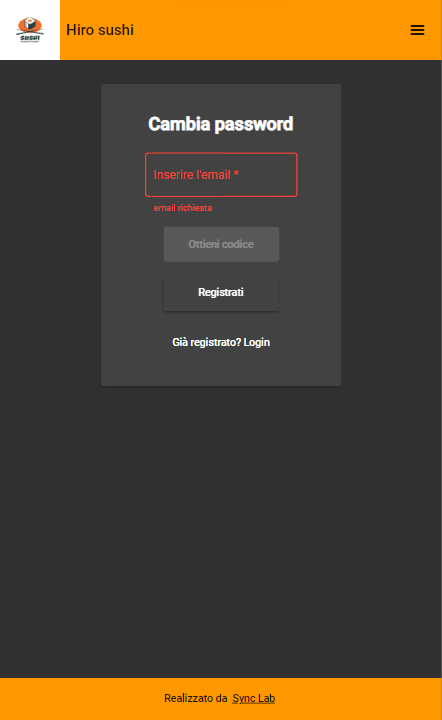
\includegraphics[scale=.5]{cambiapass2.png}
    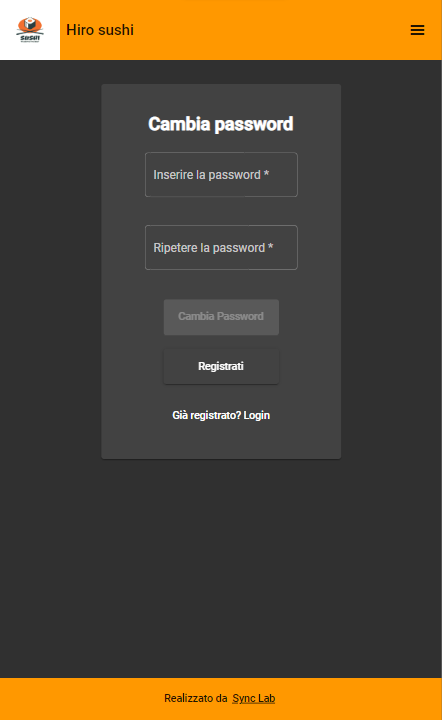
\includegraphics[scale=.5]{cambiapass3.png}
    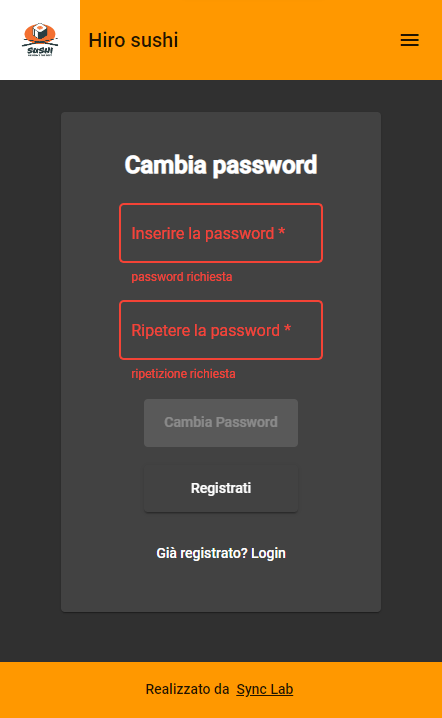
\includegraphics[scale=.5]{cambiapass4.png}
    \caption{Maschere cambia password e cambia password con i campi errati  SushiLab}
\end{figure}
\pagebreak

\subsubsection{Area Personale}
Viene mostrata l'area personale dell'utente dove si può vedere i dati dell'utente.
\textbf{Funzionalità:}
\begin{itemize}
    \item L'utente può effettuare il logout;
    \item L'utente può andare nella sezione di blacklist ingredienti per inserire o rimuovere delle allergeni o preferenze.
\end{itemize}
\begin{figure}[H]
    \centering
    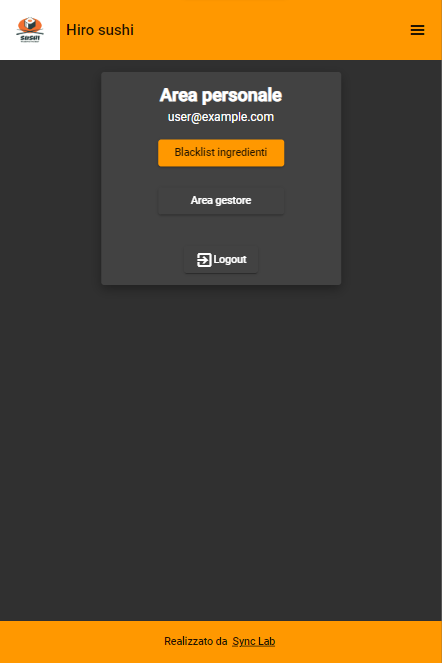
\includegraphics[scale=.6]{personale.png}
    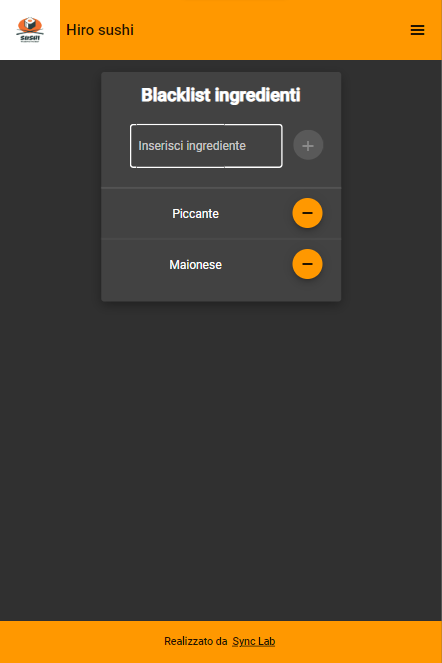
\includegraphics[scale=.6]{blacklist.png}
    \caption{Maschera area personae e blacklist SushiLab}
\end{figure}